\chapter{التقسم المنصّف والخلط الوراثي والوراثة}\label{ch:b2:meiosis-heredity}

أبوان بنيّا العينين يولد لهما طفل أزرق العينين، ولا يدهش أحد؛ وطفلان
من الأبوين نفسيهما لا يتشابهان قط، ولا يدهش أحد كذلك. والأمران
ينجمان عن عملية واحدة. فعند صنع كل بويضة وكل نطفة، تسلّم خلية فيها
نسختان من كل صبغي نسخة واحدة بالضبط، تُختار عشوائيًا، بعد أن تدع
النسختين تتبادلان قطعًا. ثم يجمع كل إلقاح نصفي طقم كهذين لم يلتقيا
قط. يصف هذا الفصل تلك العملية --- \omterm{def:b2:meiosis-heredity:meiosis}{التقسم المنصّف} --- وقواعد الوراثة
الناجمة عنها: نسب مندل واستثناءاتها، وارتباط المورّثات التي تتشارك
صبغيًا والخرائط التي يرسمها ذلك الارتباط، والوراثة الخاصة \omterm{prop:b2:meiosis-heredity:sexlinked}{للصبغيات
الجنسية} وللعضيات.

\section{التقسم المنصّف}

\begin{definition}[التقسم المنصّف]\label{def:b2:meiosis-heredity:meiosis}
\index{تقسم منصّف}\index{فردي الصيغة}\index{ثنائي الصيغة}
الخلية \emph{الثنائية الصيغة} ($2n$) تحمل صبغيين
\emph{متماثلين} من كل صنف، واحدًا من كل أب، متشابهين في محتوى
المورّثات لا في الأليلات بالضرورة. و\emph{التقسم المنصّف} هو
الانقسامان اللذان يحولان خلية ثنائية الصيغة إلى أربع خلايا
\emph{فردية الصيغة} ($n$)، لكل منها صبغي واحد من كل صنف. ويسبقه نسخ
واحد، فيدخل كل صبغي في صورة كروماتيدتين شقيقتين؛ ويفصل الانقسام
الأول \emph{المتماثلات} (وهو اختزالي)، ويفصل الثاني
\emph{الكروماتيدات الشقيقة} (وهو متساوٍ)، كما يفعل التقسم الخيطي.
وعند الحيوانات يصنع التقسم المنصّف الأعراس؛ وعند النباتات والفطريات
يصنع الأبواغ (\cref{ch:b2:plant-life-cycles})؛ وهو في كل كائن جنسي
الخطوة التي تنصّف عدد الصبغيات ليستطيع الإلقاح مضاعفته من جديد.
\end{definition}

\begin{proposition}[المراحل]\label{prop:b2:meiosis-heredity:stages}
\index{الطور التمهيدي I}\index{التزاوج الصبغي}\index{تصالب}\index{تعابر}
\emph{\omterm{prop:b2:meiosis-heredity:stages}{الطور التمهيدي I}} طويل، وفيه يقع الخلط. فتتكثف الصبغيات
المنسوخة؛ ويجد كل واحد متماثله ويتزاوج معه مورّثةً بمورّثة
(\emph{\omterm{prop:b2:meiosis-heredity:stages}{التزاوج الصبغي}})، ويمسكهما سلّم بروتيني هو \emph{المعقد
التزاوجي}، فيتكون \emph{ثنائي تكافؤ} من أربع كروماتيدات؛ وتنكسر
كروماتيدات غير شقيقة وتلتحم من جديد عند نقاط متطابقة
(\emph{التعابر})، مرة إلى مرات في ثنائي التكافؤ الواحد؛ وحين ينحل
المعقد تبقى المتماثلات متصلة عند نقاط التبادل هذه وحدها، وهي مرئية
بصورة \emph{تصالبات}. و\emph{الطور الاستوائي I}: تصطف ثنائيات
التكافؤ على المغزل، ويتوجه كل زوج عشوائيًا --- فالمتماثل الأمومي
نحو قطب أو آخر مستقلًا عن كل زوج سواه. و\emph{الطور الانفصالي I}:
تنفصل المتماثلات وتبقى الكروماتيدات الشقيقة معًا؛ فيتلقى كل قطب $n$
صبغيًا من كروماتيدتين لكل منها. و\emph{الطور النهائي I}، ثم،
عادةً دون نسخ، \emph{\omterm{def:b2:meiosis-heredity:meiosis}{التقسم المنصّف} II}: تصطف الصبغيات $n$ فرادى،
وتنفصل الكروماتيدات الشقيقة، فتنتج أربع نوى فردية الصيغة. ويستغرق
\omterm{def:b2:meiosis-heredity:meiosis}{التقسم المنصّف} الأول ساعات إلى عقود (فالبويضة البشرية تتوقف في
\omterm{prop:b2:meiosis-heredity:stages}{الطور التمهيدي I} من قبل الولادة حتى الإباضة)؛ أما \omterm{def:b2:meiosis-heredity:meiosis}{التقسم المنصّف}
الثاني فيستغرق ساعة.
\end{proposition}

\begin{omfigure}
\begin{tikzpicture}[every node/.style={font=\scriptsize}]
  % helper: cell outline at (x,y)
  \foreach \x/\lab in {0/{الطور التمهيدي I: تزاوج وتعابر}, 3.2/{الطور الاستوائي I: ثنائيات تكافؤ مصطفة}, 6.4/{الطور الانفصالي I: افتراق المتماثلات}, 9.6/{التقسم المنصّف II: افتراق الكروماتيدات}}
    { \draw[thick] (\x+1.2,0) circle (1.15); \node[below, align=center, text width=2.8cm] at (\x+1.2,-1.2) {\lab}; }
  % prophase I: one bivalent with chiasma
  \draw[very thick, omDef] (0.8,-0.5) -- (0.8,0.5); \draw[very thick, omDef] (1.0,-0.5) -- (1.0,0.5);
  \draw[very thick, omThm] (1.4,-0.5) -- (1.4,0.5); \draw[very thick, omThm] (1.6,-0.5) -- (1.6,0.5);
  \draw[very thick, omDef] (1.0,0.1) -- (1.4,-0.1); \draw[very thick, omThm] (1.4,0.1) -- (1.0,-0.1);
  \fill[white] (0.9,-0.03) rectangle (1.5,0.03);
  \draw[very thick, omDef] (1.0,0.1) -- (1.4,-0.1); \draw[very thick, omThm] (1.4,0.1) -- (1.0,-0.1);
  \node[omExo!60!black] at (1.2,-0.85) {تصالب};
  % metaphase I: two bivalents on the plate, spindle
  \begin{scope}[xshift=3.2cm]
    \draw[gray, dashed] (1.2,-1.0) -- (1.2,1.0);
    \foreach \y in {0.45,-0.45} {
      \draw[very thick, omDef] (0.95,\y-0.25) -- (0.95,\y+0.25); \draw[very thick, omDef] (1.08,\y-0.25) -- (1.08,\y+0.25);
      \draw[very thick, omThm] (1.32,\y-0.25) -- (1.32,\y+0.25); \draw[very thick, omThm] (1.45,\y-0.25) -- (1.45,\y+0.25);
    }
    \draw[gray] (0.15,0) -- (0.95,0.45); \draw[gray] (0.15,0) -- (0.95,-0.45);
    \draw[gray] (2.25,0) -- (1.45,0.45); \draw[gray] (2.25,0) -- (1.45,-0.45);
  \end{scope}
  % anaphase I
  \begin{scope}[xshift=6.4cm]
    \foreach \y in {0.45,-0.45} {
      \draw[very thick, omDef] (0.45,\y-0.25) -- (0.45,\y+0.25); \draw[very thick, omDef] (0.58,\y-0.25) -- (0.58,\y+0.25);
      \draw[very thick, omThm] (1.82,\y-0.25) -- (1.82,\y+0.25); \draw[very thick, omThm] (1.95,\y-0.25) -- (1.95,\y+0.25);
    }
    \draw[->, gray] (1.2,0) -- (0.75,0); \draw[->, gray] (1.2,0) -- (1.65,0);
  \end{scope}
  % meiosis II: four cells
  \begin{scope}[xshift=9.6cm]
    \foreach \p/\c in {(0.75,0.5)/omDef,(1.65,0.5)/omDef,(0.75,-0.5)/omThm,(1.65,-0.5)/omThm} {
      \draw[thick, gray!60] \p circle (0.38);
      \draw[very thick, \c] \p ++(-0.12,-0.2) -- ++(0,0.4);
      \draw[very thick, \c] \p ++(0.12,-0.2) -- ++(0,0.4);
    }
  \end{scope}
\end{tikzpicture}

{\small \omterm{def:b2:meiosis-heredity:meiosis}{التقسم المنصّف} عند زوجين من المتماثلات (الأمومي بالأزرق،
والأبوي بالأحمر، ولكل منهما كروماتيدتان). تتزاوج المتماثلات وتتبادل
القطع في \omterm{prop:b2:meiosis-heredity:stages}{الطور التمهيدي I}، وتصطف ثنائيات تكافؤ في الطور الاستوائي
I، وتنفصل في الطور الانفصالي I؛ ثم يفصل \omterm{def:b2:meiosis-heredity:meiosis}{التقسم المنصّف} الثاني
الكروماتيدات إلى أربع خلايا فردية الصيغة.}
\end{omfigure}

\begin{omfigure}
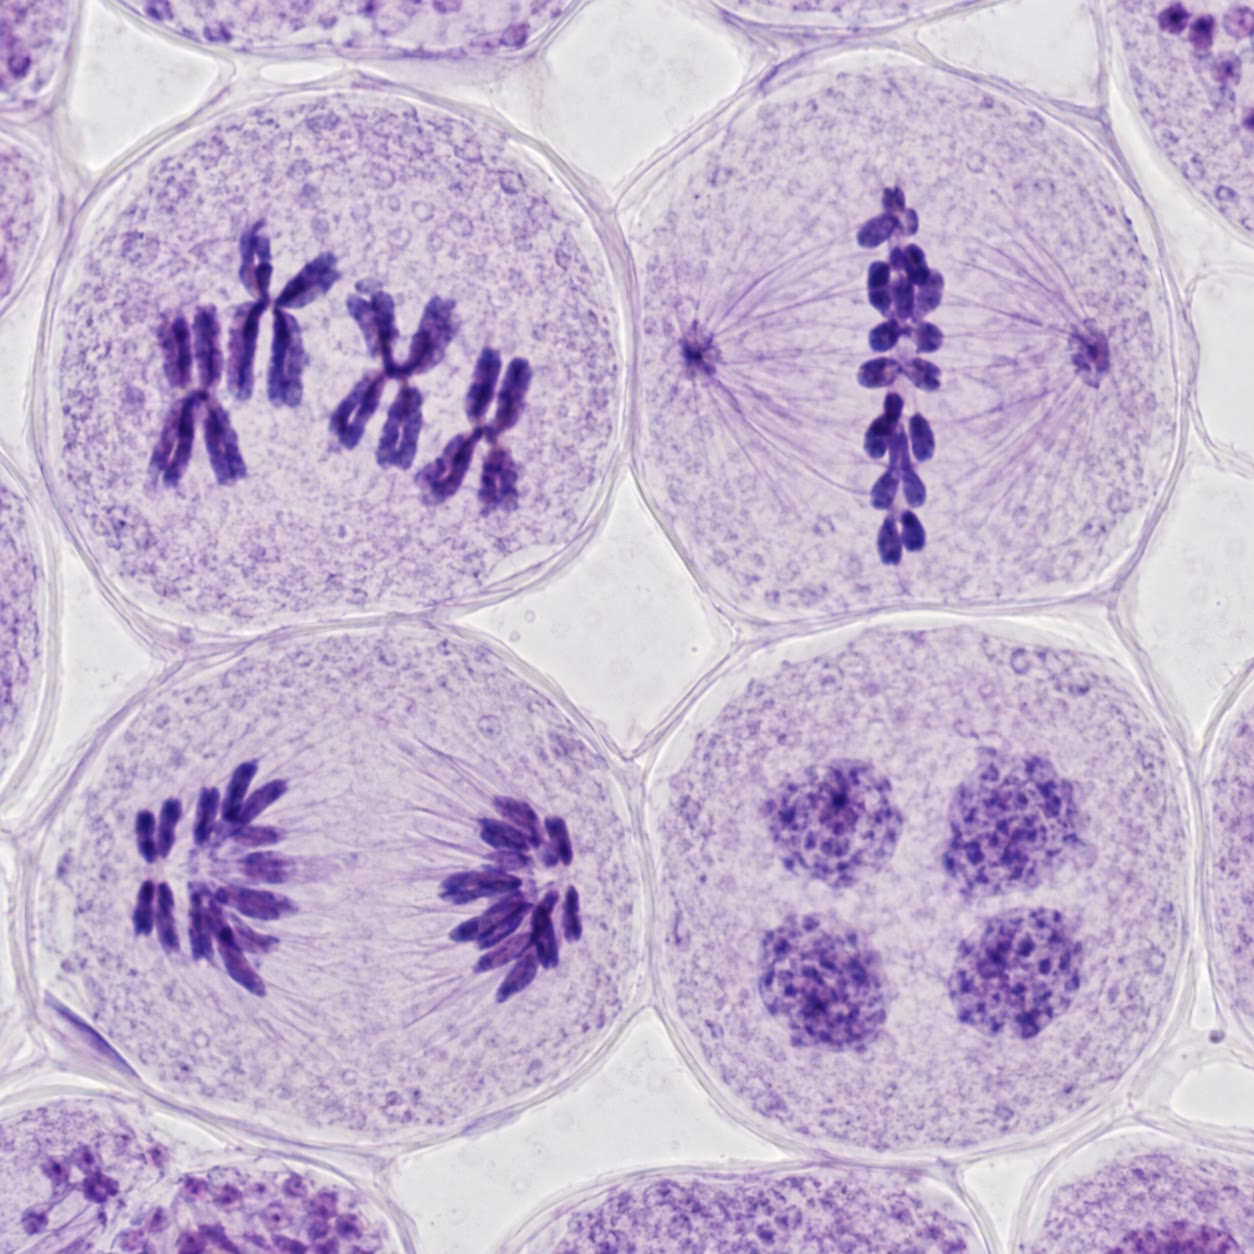
\includegraphics[width=0.5\linewidth]{images/book4/ai/b4-04-lily-meiosis.jpg}

{\small \omterm{def:b2:meiosis-heredity:meiosis}{التقسم المنصّف} في متك زنبقة: ثنائيات تكافؤ في أواخر \omterm{prop:b2:meiosis-heredity:stages}{الطور
التمهيدي I}، وصفيحة الطور الاستوائي I، والطور الانفصالي I، ونوى
الرباعية الأربع.}
\end{omfigure}

\begin{theorem}[كم من الخلط يصنع التقسم المنصّف]\label{thm:b2:meiosis-heredity:mixing}
\index{التوزع المستقل}\index{إعادة التركيب الوراثي}
عند كائن له $n$ زوجًا من الصبغيات، يعطي التوجه العشوائي لثنائيات
التكافؤ في الطور الاستوائي I عدد $2^n$ تركيبًا ممكنًا من الصبغيات
الأمومية والأبوية في العروس ---
أي $2^{23} \approx 8.4$ مليون عند الإنسان --- و$2^{2n}$ في اللاقحة.
ويضاعف التعابر هذا: فمع نحو $k$ تصالبًا في ثنائي التكافؤ، كل منها في
موضع متغير، يصير عدد الأعراس المتميزة غير محدود عمليًا، ولا تتطابق
عروسان من أعراس شخص واحد أبدًا. و\emph{إعادة التركيب} --- أي
التراكيب الجديدة من الأليلات --- تنشأ من الأمرين معًا: \omterm{thm:b2:meiosis-heredity:mixing}{فالتوزع
المستقل} يخلط الصبغيات كلها، والتعابر يخلط المورّثات داخل الصبغي
الواحد.
\end{theorem}
\begin{proof}
يتوجه كل ثنائي تكافؤ مستقلًا بنتيجتين اثنتين، فيعطي $n$ ثنائي تكافؤ
عدد $2^n$ تركيبًا، كلها متساوية الاحتمال. ويسهم كل من الأبوين بعروس
كهذه، فيكون للاقحة $2^n\times
2^n$ تركيبًا. والتعابر في موضع متميز من صبغي طوله $L$ زوج أسس يستطيع
إنتاج ما رتبته $L$ كروماتيدة معادة التركيب متميزة في ثنائي التكافؤ،
فينمو عدد النواتج المتميزة على صورة $L^k$ في الصبغي الواحد، وهو رقم فلكي
من أجل $L \sim 10^8$.
\end{proof}
\begin{proof}[شواهد]
استعمل كرايتون ومكلينتوك (1931) صبغي ذرة رقم 9 يحمل علامتين خلويتين
مرئيتين (عقدة في طرف، وقطعة منقولة في الطرف الآخر) ومورّثتين بينهما
(حبة ملونة/عديمة اللون، وسويداء شمعية/نشوية). فوجدا بين الخلف أن كل
نبات ذي زوج أليلات معاد التركيب له أيضًا زوج علامات خلوية معاد
التركيب --- عقدة بلا نقل أو العكس --- وهو ما أثبت أن \omterm{thm:b2:meiosis-heredity:mixing}{إعادة التركيب
الوراثي} تبادل فيزيائي لقطع صبغية.
\end{proof}

\begin{omfigure}
\begin{tikzpicture}[every node/.style={font=\scriptsize}]
  \foreach \dx/\lab/\ca/\cb/\gam in {0/{التوجه 1}/omDef/omThm/{أعراس AB وab}, 6.2/{التوجه 2}/omThm/omDef/{أعراس Ab وaB}} {
    \begin{scope}[xshift=\dx cm]
      \draw[gray, dashed] (0,-1.1) -- (3.2,-1.1);
      \node[anchor=south] at (1.6,0.6) {\lab};
      % pair 1 (long): A above the plate, a below
      \draw[very thick, omDef] (0.7,-0.95) -- (0.7,-0.25); \node[omDef, anchor=south] at (0.7,-0.2) {A};
      \draw[very thick, omThm] (0.7,-1.25) -- (0.7,-1.95); \node[omThm, anchor=north] at (0.7,-2.0) {a};
      % pair 2 (short): B or b above depending on orientation
      \draw[very thick, \ca] (2.3,-0.85) -- (2.3,-0.35);
      \draw[very thick, \cb] (2.3,-1.35) -- (2.3,-1.85);
      \node[anchor=north] at (1.6,-2.4) {\gam};
    \end{scope}
  }
  \node[omDef, anchor=south] at (2.3,-0.3) {B}; \node[omThm, anchor=north] at (2.3,-1.9) {b};
  \node[omThm, anchor=south] at (8.5,-0.3) {b}; \node[omDef, anchor=north] at (8.5,-1.9) {B};
  \node[anchor=north, align=center] at (4.7,-3.0) {كل توجه متساوي الاحتمال:\\أعراس AB وab وAb وaB بأعداد متساوية --- أي التوزع المستقل};
\end{tikzpicture}

{\small \omterm{thm:b2:meiosis-heredity:mixing}{التوزع المستقل}. عند زوجي صبغيات (A/a على أحدهما، وB/b على
الآخر)، يكون التوجهان الممكنان لثنائيي التكافؤ في الطور الاستوائي I
متساويي الاحتمال، فتظهر تراكيب الأليلات الأربعة بأعداد متساوية بين
الأعراس.}
\end{omfigure}

\section{التحليل المندلي}

\begin{definition}[مفردات التهجين]\label{def:b2:meiosis-heredity:vocabulary}
\index{أليل}\index{نمط وراثي}\index{نمط ظاهري}\index{سائد}\index{متنحٍّ}\index{متماثل اللواقح}\index{متغاير اللواقح}
\emph{المورّثة} شريط من الصبغي؛ و\emph{أليلاتها} هي متغيراتها
التسلسلية؛ و\emph{الموقع} هو مكانها. ويحمل الفرد \omterm{def:b2:meiosis-heredity:meiosis}{الثنائي الصيغة}
أليلين في كل موقع: فنمطه \emph{الوراثي} إما
\emph{متماثل اللواقح} ($AA$، $aa$) أو \emph{متغاير اللواقح} ($Aa$).
و\emph{النمط الظاهري} هو الصفة المرصودة. ويكون الأليل \emph{سائدًا}
حين يظهر متغاير اللواقح نمطه الظاهري، و\emph{متنحيًا} حين لا يظهر
إلا عند متماثل اللواقح؛ والتمييز صفة لزوج الأليلات وللصفة المرصودة،
لا للأليل وحده --- فمعظم الأليلات المتنحية أليلات فاقدة للوظيفة،
تختفي لأن نسخة عاملة واحدة تكفي. و\emph{السلالة النقية} تورّث بصدق
(متماثلة اللواقح)؛ و\emph{التهجين الاختباري} يزاوج فردًا ذا نمط ظاهري
سائد مع متماثل لواقح متنحٍّ، فيكشف خلفه أليلات أعراسه مباشرة.
\end{definition}

\begin{theorem}[نسب مندل]\label{thm:b2:meiosis-heredity:mendel}
\index{قوانين مندل}\index{تهجين أحادي}\index{تهجين ثنائي}
لمّا كان أليلا \omterm{def:b2:meiosis-heredity:vocabulary}{متغاير اللواقح} $Aa$ ينفصلان إلى أعراس مختلفة بأعداد
متساوية (في الطور الانفصالي I)، أعطى التهجين \emph{الأحادي}
$Aa \times Aa$ أنماطًا وراثية $\tfrac14 AA : \tfrac12 Aa :
\tfrac14 aa$، وأنماطًا ظاهرية $3 : 1$ إذا كان $A$ سائدًا؛ وأعطى
التهجين الاختباري $Aa \times aa$ نسبة $1 : 1$. ولمّا كانت أليلات
مورّثات على صبغيات مختلفة تتوزع مستقلة (في الطور الاستوائي I)، صنع
\emph{الثنائي} $AaBb$ أربعة أصناف من الأعراس بأعداد متساوية، وأعطى
التهجين $AaBb \times AaBb$ أنماطًا ظاهرية $9 : 3 : 3 : 1$، وأعطى
التهجين الاختباري $AaBb \times aabb$ نسبة $1 : 1 : 1 : 1$. ومن أجل
$k$ موقعًا \omterm{def:b2:meiosis-heredity:vocabulary}{متغاير اللواقح} مستقلًا، يكون عدد أصناف الأعراس $2^k$
وتكون النسبة الظاهرية جداء $k$ نسبة $3 : 1$.
\end{theorem}
\begin{proof}
الانفصال: أعراس \omterm{def:b2:meiosis-heredity:vocabulary}{متغاير اللواقح} هي $\tfrac12 A$
و$\tfrac12 a$؛ ومع إلقاح عشوائي تكون أنماط اللاقحة الوراثية هي
الجداءات $(\tfrac12 A + \tfrac12 a)^2 = \tfrac14 AA + \tfrac12 Aa +
\tfrac14 aa$. والاستقلال: أعراس $AaBb$ هي $(\tfrac12 A
+ \tfrac12 a)(\tfrac12 B + \tfrac12 b)$، أي أربعة أصناف عند
$\tfrac14$؛ وتتضارب الأنماط الظاهرية الثنائية $(\tfrac34 A\_ + \tfrac14 aa)
(\tfrac34 B\_ + \tfrac14 bb)$، فتعطي $\tfrac{9}{16}, \tfrac{3}{16},
\tfrac{3}{16}, \tfrac{1}{16}$. وكل عامل انفصال مستقل واحد، فيعطي $k$
موقعًا جداء $k$ عاملًا.
\end{proof}
\begin{proof}[شواهد]
هجّن مندل (1866) سلالات نقية من البازلاء تختلف في صفة واحدة ---
بذرة ملساء أو مجعدة، وفلقة صفراء أو خضراء، وزهرة أرجوانية أو بيضاء،
وساق طويلة أو قزمة وثلاث صفات أخرى --- فوجد في كل حالة جيلًا أول
موحدًا وجيلًا ثانيًا ينفصل قريبًا من $3 : 1$: 5474 ملساء إلى 1850
مجعدة ($2.96 :
1$)، و6022 صفراء إلى 2001 خضراء ($3.01 : 1$)، و705 أرجوانية إلى 224
بيضاء ($3.15 : 1$). وفي تهجينات الصفتين وجد $315 : 108 : 101 :
32$ (أي $9 : 3 : 3 : 1$)، وبإنماء الجيل الثاني بيّن أن الصنف \omterm{def:b2:meiosis-heredity:vocabulary}{السائد}
صنفان، ثلثه نقي وثلثاه ينفصلان. أما الصبغيات التي تفسر هذه النسب
فوُجدت بعد أربعين سنة.
\end{proof}

\begin{omfigure}
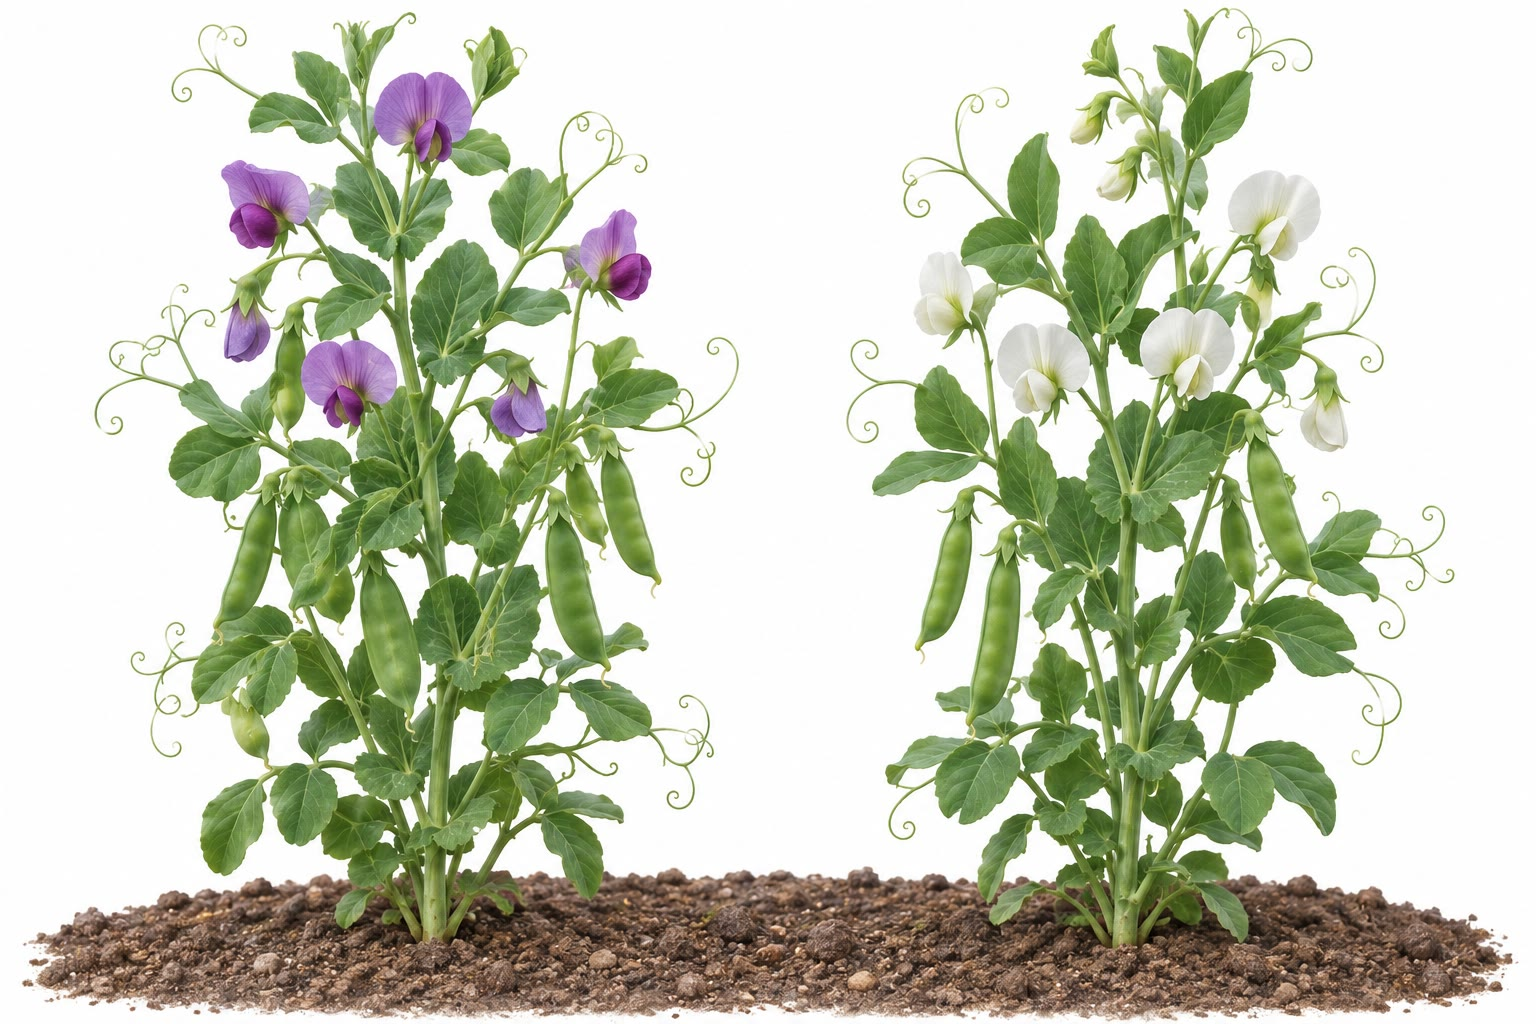
\includegraphics[width=0.58\linewidth]{images/book4/ai/b4-04-pea-flowers.jpg}

{\small نبات بازلاء أرجواني الزهر وآخر أبيض الزهر: أحد أزواج الصفات
السبعة التي أسس عليها مندل علم الوراثة. والهجين الأرجواني الزهر،
إذا لُقّح ذاتيًا، أعطى نحو ثلاث أرجوانيات إلى بيضاء واحدة.}
\end{omfigure}

\begin{method}[اختبار نسبة بالمقدار $\chi^2$]\label{met:b2:meiosis-heredity:chisquare}
\index{اختبار مربع كاي}
للبت في موافقة الأعداد المرصودة $O_i$ نسبةً مفترضة:
\begin{enumerate}
  \item احسب الأعداد المنتظرة $E_i$ من النسبة ومن المجموع.
  \item احسب $\chi^2 = \sum_i (O_i - E_i)^2/E_i$.
  \item عُدّ درجات الحرية: عدد الأصناف ناقص واحد.
  \item قارن بالقيمة الحرجة عند مستوى \qty{5}{\%}:
        $3.84$ لدرجة حرية واحدة، و$5.99$ لدرجتين، و$7.81$ لثلاث،
        و$9.49$ لأربع. فإذا كان $\chi^2$ دونها كانت المعطيات
        متوافقة مع النسبة؛ وإذا كان فوقها رُفضت النسبة --- إذ
        كان الانحراف ليقع مصادفةً في أقل من تجربة واحدة من عشرين.
\end{enumerate}
وعند أزهار مندل، $705 : 224$ في مقابل $3 : 1$: يكون $E = 696.75,
232.25$؛ و$\chi^2 = 0.098 + 0.293 = 0.39 < 3.84$. (أما التوزيع الذي
وراء القيم الحرجة فمشتق في إحصاء سلسلة الرياضيات؛ والجدول هنا أداة.)
\end{method}

\begin{proposition}[ما وراء النسب البسيطة]\label{prop:b2:meiosis-heredity:extensions}
\index{سيادة ناقصة}\index{سيادة مشتركة}\index{تفوق مورّثي}\index{أليل مميت}
تتغير النسب، ولا تتغير الآلية، حين: تُظهر الأليلات
\emph{\omterm{prop:b2:meiosis-heredity:extensions}{سيادة ناقصة}} (فحنك السبع الأحمر $\times$ الأبيض يعطي ورديًا،
والجيل الثاني $1 : 2 : 1$)؛ أو تكون الأليلات
\emph{مشتركة السيادة}، فيُعبَّر عنها كلها (زمرة الدم $AB$: \omterm{def:b2:meiosis-heredity:vocabulary}{متغاير
اللواقح} $I^AI^B$ يصنع المستضدين معًا؛ وقد يكون للموقع \emph{أليلات
متعددة}: $I^A$ و$I^B$ و$i$)؛ أو يكون \omterm{def:b2:meiosis-heredity:vocabulary}{الأليل} \emph{مميتًا} في حال
تماثل اللواقح (الفئران الصفراء: أصفر $\times$ أصفر يعطي $2$ أصفر إلى
$1$ رمادي مخطط، إذ يموت $\tfrac14 YY$ أجنّة)؛ أو تعمل مورّثتان في
مسلك واحد (\emph{\omterm{prop:b2:meiosis-heredity:extensions}{التفوق المورّثي}}: ففي تهجين $9 : 3 : 3 : 1$ قد لا
يتميز متنحي المورّثتين عن أحد متنحيي المورّثة الواحدة، فتصير النسبة
$9 : 3 : 4$، كما في الفئران المهقاء، أو قد يلزم السائدان معًا \omterm{def:b2:meiosis-heredity:vocabulary}{للنمط
الظاهري}، فتصير $9 : 7$، كما في بازلاء الزينة الأرجوانية التي تحتاج
إلى إنزيمين لصنع صبغتها)؛ أو تضيف مورّثات كثيرة كل منها قليلًا إلى
صفة متصلة (الطول، والمردود)، وهذه هي الوراثة الكمية في
\cref{ch:b2:population-genetics}. وقراءة النسبة رجوعًا إلى آلية هي
حرفة الوراثة اليومية.
\end{proposition}

\section{الارتباط والخرائط الوراثية}

\begin{definition}[الارتباط وتواتر إعادة التركيب]\label{def:b2:meiosis-heredity:linkage}
\index{ارتباط}\index{تواتر إعادة التركيب}\index{سنتيمورغان}
المورّثتان على الصبغي نفسه \emph{مرتبطتان}: فأليلاتهما تنزع إلى
السفر معًا إلى الأعراس، ويصنع الثنائي
$AB/ab$ أعراسًا \emph{أبوية} ($AB$، $ab$) أكثر من الأعراس
\emph{المعادة التركيب} ($Ab$، $aB$). ولا تنشأ معادات التركيب إلا حين
يقع تعابر بين الموقعين، فيقيس تواترها $r$ --- المعدود مباشرة في
تهجين اختباري --- المسافةَ: ويتراوح $r$ من 0 (ارتباط تام) إلى
$\tfrac12$ (مورّثتان متباعدتان جدًا، أو على صبغيين مختلفين، فتتوزعان
مستقلتين). ووحدة \emph{المسافة على الخريطة} هي \emph{السنتيمورغان}
(cM): فالمقدار \qty{1}{cM} هو \qty{1}{\%} إعادة تركيب عند مورّثتين شديدتي
الارتباط؛ و\qty{1}{cM} عند الإنسان نحو مليون زوج أسس. وكان الارتباط أول
برهان على أن المورّثات تقع على خط في الصبغي.
\end{definition}
\begin{proof}[شواهد]
وجد مورغان (1911) أن مورّثتي العين البيضاء والجناح الصغير عند
الذبابة، وكلتاهما على الصبغي X، لا تتوزعان مستقلتين: فأعطى تهجين
اختباري \qty{37}{\%} من معادات التركيب بدل \qty{50}{\%}،
وأعطت أزواج أخرى نسبًا أخرى قابلة للتكرار. ثم أدرك ستيرتيفانت
(1913)، وكان طالبًا جامعيًا، أن التواترات إن كانت تقيس مسافات وجب
أن تتجمع: فرسم من التواترات الثنائية لست مورّثات مرتبطة بالصبغي X
أول خريطة وراثية، وكانت المسافات، في حدود الخطأ، تجميعية على خط.
\end{proof}

\begin{omfigure}
\begin{tikzpicture}[every node/.style={font=\scriptsize}]
  % bivalent with crossover between A and B
  \draw[very thick, omDef] (0,1.2) -- (2.0,1.2) -- (3.0,0.6) -- (5,0.6);
  \draw[very thick, omDef] (0,1.5) -- (5,1.5);
  \draw[very thick, omThm] (0,0.3) -- (2.0,0.3) -- (3.0,0.9) -- (5,0.9);
  \draw[very thick, omThm] (0,0) -- (5,0);
  \node[omDef, above] at (0.8,1.5) {A}; \node[omDef, above] at (4.3,1.5) {B};
  \node[omThm, below] at (0.8,0) {a}; \node[omThm, below] at (4.3,0) {b};
  \node[anchor=south, gray] at (2.5,1.85) {تعابر بين موقعي A وB};
  % products
  \draw[->, thick, gray] (5.4,0.75) -- (6.2,0.75);
  \node[anchor=west, align=left] at (6.4,1.45) {\textcolor{omDef}{A\,B} \quad أبوية};
  \node[anchor=west, align=left] at (6.4,0.95) {\textcolor{omDef}{A}\,\textcolor{omThm}{b} \quad معادة التركيب};
  \node[anchor=west, align=left] at (6.4,0.5) {\textcolor{omThm}{a}\,\textcolor{omDef}{B} \quad معادة التركيب};
  \node[anchor=west, align=left] at (6.4,0.0) {\textcolor{omThm}{a\,b} \quad أبوية};
  \node[anchor=west, align=left, text width=5.6cm] at (6.4,-0.9) {تعابر واحد بين الموقعين في كسر $c$ من التقسمات المنصّفة: فالأعراس المعادة التركيب $r = c/2$، إذ لا تتبادل إلا اثنتان من الكروماتيدات الأربع};
\end{tikzpicture}

{\small إعادة التركيب بين موقعين مرتبطين. التعابر بينهما في ثنائي
تكافؤ يبادل الأليلات على اثنتين من الكروماتيدات الأربع؛ وتُعدّ
الأعراس المعادة التركيب في تهجين اختباري، ويقيس تواترها المسافة.}
\end{omfigure}

\begin{method}[رسم خريطة مورّثتين مرتبطتين]\label{met:b2:meiosis-heredity:twopoint}
\begin{enumerate}
  \item هجّن سلالتين نقيتين للحصول على الثنائي؛ ولاحظ أي الأليلات
        تلقاها معًا (أي تراكيبه الأبوية،
        \emph{التزاوج} $AB/ab$ أو \emph{التنافر} $Ab/aB$).
  \item هجّنه اختباريًا مع متنحي المورّثتين وصنّف الخلف: فالصنفان
        الأكثر عددًا أبويان، والأقلان معادا التركيب.
  \item $r = $ معادات التركيب $/$ المجموع؛ والمسافة $100\,r$ \omterm{def:b2:meiosis-heredity:linkage}{سنتيمورغان}.
  \item وتحقق من الاستقلال أولًا: فإذا كانت الأصناف الأربعة متساوية
        ($\chi^2$ في مقابل $1 : 1 : 1 : 1$) كانت المورّثتان غير مرتبطتين.
\end{enumerate}
\end{method}

\begin{theorem}[دالة الرسم عند هالدين]\label{thm:b2:meiosis-heredity:haldane}
\index{دالة الرسم}
يقلّل \omterm{def:b2:meiosis-heredity:linkage}{تواتر إعادة التركيب} من تقدير المسافة عند المورّثات المتباعدة،
لأن تعابرين بينهما يعيدان التركيب الأبوي. فإذا وقعت التعابرات
مستقلة على امتداد الصبغي (بلا تداخل)، وكان $d$ المسافة على الخريطة
بالمورغان (أي العدد المنتظر للتعابرات في الكروماتيدة الواحدة)، كان
كسر إعادة التركيب
\[
r = \tfrac12\,\bigl(1 - e^{-2d}\bigr), \qquad d = -\tfrac12\ln(1 - 2r),
\]
فيكون $r \approx d$ عند $d$ الصغيرة، ويكون $r \to \tfrac12$ كلما
كبر $d$؛ والقيمة $r = 0.40$ تقابل \qty{80}{cM}، و\qty{50}{cM}
تعطي $r = 0.32$. وتُظهر الصبغيات الحقيقية \emph{تداخلًا} --- إذ
يجعل تعابرٌ تعابرًا آخر قريبًا أقل احتمالًا --- وهو ما يقرّب $r$ من
$d$ أكثر مما يتنبأ هالدين على المسافات القصيرة.
\end{theorem}
\begin{proof}
ليكن $d$ المسافة على الخريطة، أي العدد المنتظر للتعابرات في
الكروماتيدة الواحدة ضمن المجال؛ ولمّا كان كل تعابر يشمل اثنتين من
الكروماتيدات الأربع، حمل ثنائي التكافؤ كله عددًا بواسونيًا من
التعابرات متوسطه $2d$ في المجال، وكان احتمال ألا يحمل أيًا منها
$e^{-2d}$. وإذا حمل واحدًا على الأقل، شمل كل تعابر كروماتيدةً معينة
مستقلًا باحتمال
$\tfrac12$، فتكون تلك الكروماتيدة قد تبادلت عددًا فرديًا من
المرات --- أي صارت معادة التركيب --- باحتمال $\tfrac12$ بالضبط،
مهما كان عدد التعابرات. ومنه $r = \tfrac12\,(1 -
e^{-2d})$؛ وبالقلب نجد $d$. وعند $d$ الصغيرة يكون $r \approx d$؛ وحين
يؤول $d \to \infty$ يؤول $r \to \tfrac12$.
\end{proof}

\begin{omfigure}
\begin{tikzpicture}
\begin{axis}[
  width=0.72\linewidth, height=5.6cm,
  axis x line=bottom, axis y line=left,
  xmin=0, xmax=150, ymin=0, ymax=0.55,
  xlabel={المسافة على الخريطة $d$ (cM)}, ylabel={كسر إعادة التركيب $r$},
  xlabel style={font=\small, at={(axis description cs:0.5,-0.13)}, anchor=north},
  ylabel style={font=\small},
  tick label style={font=\small}, xtick={0,50,100,150}, ytick={0,0.25,0.5},
  legend style={font=\scriptsize, at={(0.97,0.1)}, anchor=south east, draw=none},
  clip=false,
]
\addplot[very thick, omDef, domain=0:150, samples=80] {0.5*(1-exp(-2*x/100))};
\addlegendentry{هالدين: $r = \tfrac12(1 - e^{-2d})$}
\addplot[thick, dashed, gray, domain=0:50, samples=2] {x/100};
\addlegendentry{$r = d$ (بلا تعابرات مضاعفة)}
\draw[dashed, gray] (axis cs:0,0.5) -- (axis cs:150,0.5);
\end{axis}
\end{tikzpicture}

{\small كسر إعادة التركيب بدلالة المسافة على الخريطة. المورّثات
المتقاربة تعيد التركيب بنسبة مسافتها؛ أما المتباعدة فلا تتجاوز
\qty{50}{\%} من إعادة التركيب مهما تباعدت، لأن التعابرات المضاعفة
تعيد التراكيب الأبوية.}
\end{omfigure}

\begin{method}[التهجين الاختباري الثلاثي النقاط]\label{met:b2:meiosis-heredity:threepoint}
\index{تهجين ثلاثي النقاط}\index{تداخل}
هجّن متغاير لواقح ثلاثيًا $ABC/abc$ مع $abc/abc$ وصنّف أصناف الخلف
الثمانية.
\begin{enumerate}
  \item الصنفان الأكبر أبويان؛ والأصغران هما
        \emph{التعابران المضاعفان}.
  \item والمورّثة التي تتبدل بين صنف أبوي وصنف التعابر المضاعف هي
        \emph{الوسطى}: وهذا يعطي الترتيب.
  \item ومن أجل كل زوج متجاور، يكون \omterm{def:b2:meiosis-heredity:linkage}{تواتر إعادة التركيب}
        (التعابرات المفردة في ذلك المجال + التعابرات المضاعفة) $/$
        المجموع، إذ إن التعابر المضاعف يعيد تركيب المجالين معًا.
  \item والتعابرات المضاعفة المنتظرة $= r_1 r_2 \times$ المجموع؛
        و\emph{معامل التصادف} هو المرصود على المنتظر،
        و\emph{التداخل} هو $1 -$ التصادف.
\end{enumerate}
\end{method}

\begin{example}[تهجين ثلاثي النقاط محلول]\label{ex:b2:meiosis-heredity:threepoint}
خلف $+++/abc \times abc/abc$: $+++$ 580، و$abc$ 592، و$++c$
45، و$ab+$ 40، و$+bc$ 89، و$a++$ 94، و$+b+$ 3، و$a+c$ 5؛ والمجموع 1448.
والأبويان $+++$ و$abc$؛ والمضاعفان $+b+$ و$a+c$؛ وبمقارنة $+++$
مع $+b+$ نجد أن المورّثة التي تبدلت هي $b$: فالترتيب $a$--$b$--$c$. ومنه $r_{ab} =
(89 + 94 + 3 + 5)/1448 = 0.132$؛ و$r_{bc} = (45 + 40 + 3 + 5)/1448 =
0.064$؛ والخريطة: $a$ --- \qty{13.2}{cM} --- $b$ --- \qty{6.4}{cM} ---
$c$. والمضاعفان المنتظران $0.132\times 0.064\times 1448 = 12.2$،
والمرصودان 8: فالتصادف $0.65$، والتداخل $0.35$.
\end{example}

\begin{omfigure}
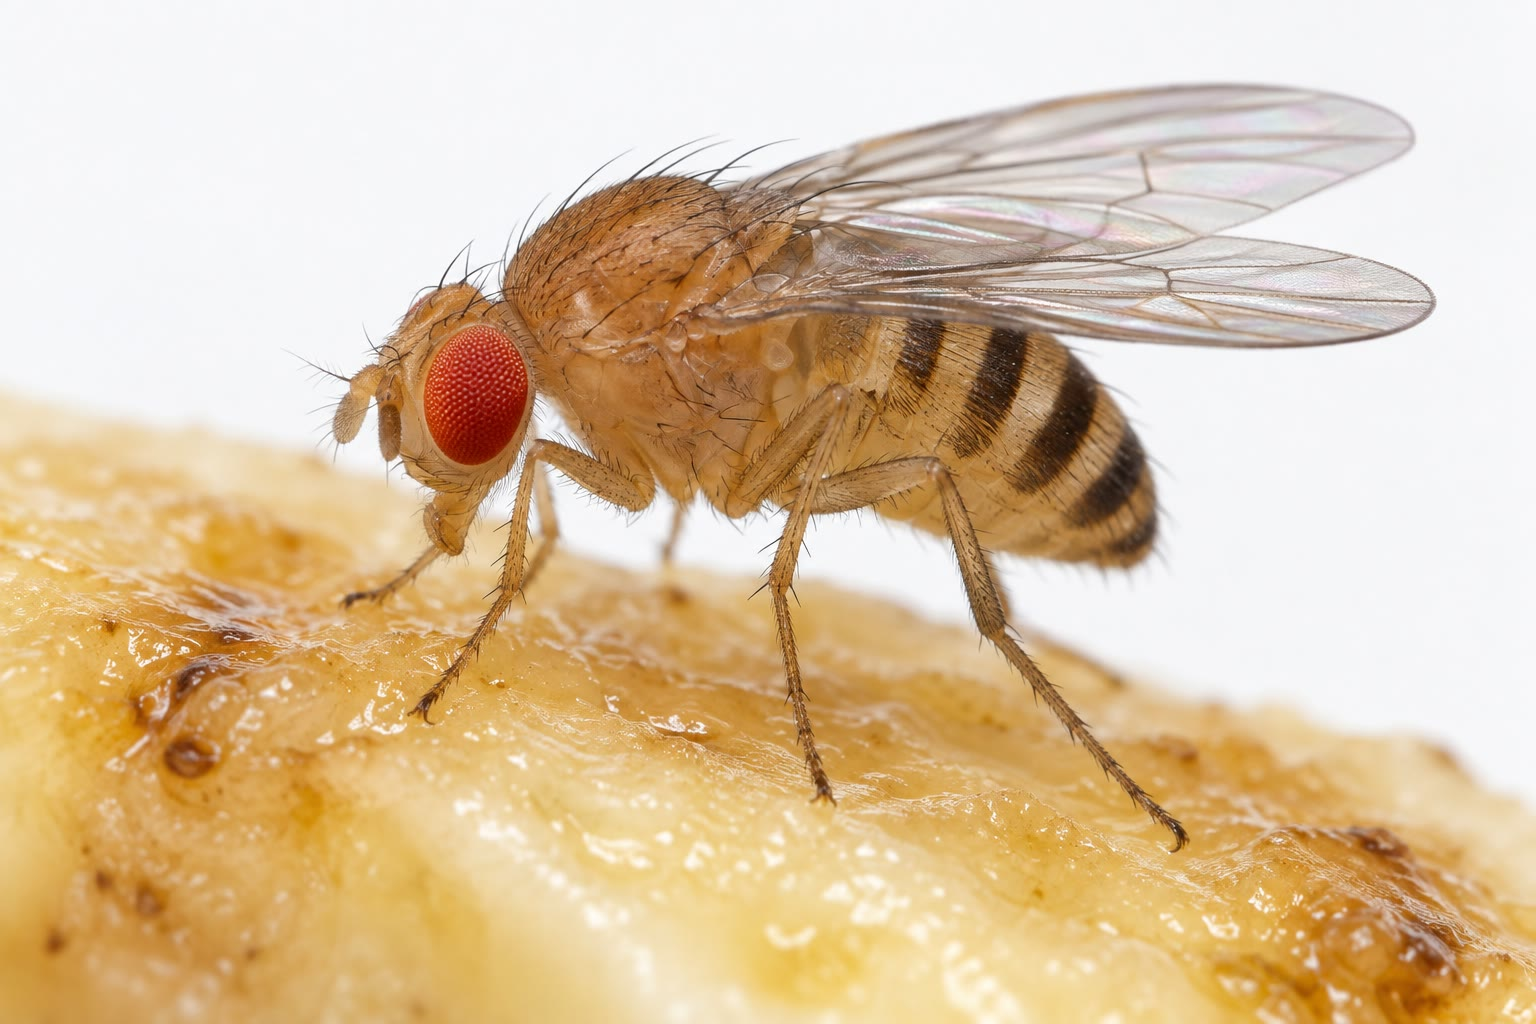
\includegraphics[width=0.5\linewidth]{images/book4/ai/b4-04-drosophila.jpg}

{\small \emph{Drosophila melanogaster}: أسبوعان لكل جيل، ومئات
الخلف، وأربعة أزواج من الصبغيات، وقرن من الطافرات --- وهي الكائن
الذي استُخرج عليه الارتباط والخرائط والوراثة المرتبطة بالجنس.}
\end{omfigure}

\section{الصبغيات الجنسية والعضيات}

\begin{proposition}[الوراثة المرتبطة بالجنس]\label{prop:b2:meiosis-heredity:sexlinked}
\index{وراثة مرتبطة بالصبغي X}\index{صبغيات جنسية}
عند الثدييات والذباب تكون الأنثى $XX$ والذكر $XY$: والصبغي $Y$ يحمل
مورّثات قليلة، فيكون للذكر نسخة واحدة من كل مورّثة مرتبطة بالصبغي $X$
(فهو \emph{فردي \omterm{def:b2:meiosis-heredity:vocabulary}{الأليل}})، ويُظهر أي \omterm{def:b2:meiosis-heredity:vocabulary}{أليل} يحمله، سائدًا كان أم
متنحيًا. والعواقب: أن التهجينين المتعاكسين يختلفان (فأنثى بيضاء
العين $\times$ ذكر أحمر العين يعطي أبناء بيض العيون وبنات حمرها؛
والتهجين المعاكس يعطي الجميع حمرًا)؛ وأن الصفة المتنحية المرتبطة
بالصبغي $X$ (عمى الألوان الأحمر--الأخضر، والناعور، وحثل دوشين العضلي)
تظهر عند الذكور في معظمها، وتنقلها أمهات حاملات غير مصابات، ولا
تنتقل قط من أب إلى ابن (فالابن يأخذ $Y$ أبيه)؛ وأن الأب ينقل $X$
إلى بناته كلهن. أما الطيور والفراشات وبعض الزواحف فتعكس الترتيب
(إناث $ZW$، وذكور $ZZ$)؛ وكثير من الزواحف يدع الحرارة تقرر؛ وعند
الثدييات يُسكت أحد صبغيي $X$ في كل خلية أنثوية عشوائيًا في مطلع
النمو، فتكون الأنثى المتغايرة اللواقح فسيفساء (كالقطة السلحفائية).
\end{proposition}
\begin{proof}[شواهد]
وجد مورغان (1910) ذكرًا واحدًا أبيض العين بين آلاف الذباب الأحمر
العيون. وبتهجينه مع إناث حمر جاء الخلف كله أحمر؛ لكن العيون البيضاء
عادت في الجيل التالي عند الذكور وحدهم، عند نصفهم. وتهجين ذكر أبيض
مع بناته الحمر أعطى عيونًا بيضاء في الجنسين. وكان النمط تمامًا ما
يُنتظر لو كانت المورّثة على الصبغي X، الذي تحمله الإناث مرتين
والذكور مرة --- وهي أول مورّثة تُنسب إلى صبغي.
\end{proof}

\begin{omfigure}
\begin{tikzpicture}[every node/.style={font=\scriptsize}]
  % pedigree: X-linked recessive
  \draw[thick, fill=gray!70] (0,0) rectangle (0.5,0.5); % affected grandfather
  \draw[thick] (1.5,0.25) circle (0.25);
  \draw[thick] (0.5,0.25) -- (1.25,0.25);
  \draw[thick] (0.875,0.25) -- (0.875,-0.5);
  \draw[thick] (0.875,-0.5) -- (3.5,-0.5);
  % children of generation I
  \draw[thick] (0.875,-0.5) -- (0.875,-0.9); \draw[thick, fill=white] (0.875,-1.15) circle (0.25); \fill (0.875,-1.15) circle (0.08);
  \draw[thick] (2.2,-0.5) -- (2.2,-0.9); \draw[thick] (1.95,-1.4) rectangle (2.45,-0.9);
  \draw[thick] (3.5,-0.5) -- (3.5,-0.9); \draw[thick, fill=white] (3.5,-1.15) circle (0.25); \fill (3.5,-1.15) circle (0.08);
  % carrier daughter marries
  \draw[thick] (-0.3,-1.15) -- (0.625,-1.15); \draw[thick] (-0.55,-1.4) rectangle (-0.05,-0.9);
  \draw[thick] (0.15,-1.15) -- (0.15,-1.9); \draw[thick] (-1.2,-1.9) -- (1.5,-1.9);
  \draw[thick] (-1.2,-1.9) -- (-1.2,-2.3); \draw[thick, fill=gray!70] (-1.45,-2.8) rectangle (-0.95,-2.3);
  \draw[thick] (-0.3,-1.9) -- (-0.3,-2.3); \draw[thick] (-0.55,-2.8) rectangle (-0.05,-2.3);
  \draw[thick] (0.6,-1.9) -- (0.6,-2.3); \draw[thick, fill=white] (0.6,-2.55) circle (0.25); \fill (0.6,-2.55) circle (0.08);
  \draw[thick] (1.5,-1.9) -- (1.5,-2.3); \draw[thick, fill=white] (1.5,-2.55) circle (0.25);
  \node[anchor=east] at (-1.8,0.25) {I};
  \node[anchor=east] at (-1.8,-1.15) {II};
  \node[anchor=east] at (-1.8,-2.55) {III};
  % legend
  \node[anchor=west, align=left] at (5,-0.4) {$\square$ ذكر \quad $\bigcirc$ أنثى};
  \draw[thick, fill=gray!70] (5.05,-1.25) rectangle (5.45,-0.85); \node[anchor=west] at (5.6,-1.05) {مصاب};
  \draw[thick] (5.25,-1.85) circle (0.2); \fill (5.25,-1.85) circle (0.07); \node[anchor=west] at (5.6,-1.85) {حامل (متغاير اللواقح)};
  \node[anchor=north west, align=left, text width=6.2cm] at (5,-2.3) {متنحٍّ مرتبط بالصبغي X: للرجل المصاب أطفال غير مصابين، وبناته كلهن يحملن الأليل، ونصف أبنائهن مصابون --- فالصفة تتخطى جيلًا وتعود عند الأحفاد};
\end{tikzpicture}

{\small \omterm{met:b2:meiosis-heredity:pedigree}{شجرة نسب} لصفة متنحية مرتبطة بالصبغي X كالناعور: لا انتقال
من أب إلى ابن، وبنات حاملات، وأحفاد مصابون.}
\end{omfigure}

\begin{method}[قراءة شجرة النسب]\label{met:b2:meiosis-heredity:pedigree}
\index{شجرة نسب}
\begin{enumerate}
  \item أبوان غير مصابين ولهما طفل مصاب: الصفة متنحية (وكلا الأبوين
        \omterm{def:b2:meiosis-heredity:vocabulary}{متغاير اللواقح}).
  \item طفل مصاب له دائمًا أب مصاب، والصفة تظهر في كل جيل: سائدة.
  \item المصابون ذكور في معظمهم، والصفة تنتقل عبر أمهات غير مصابات،
        ولا تنتقل من أب إلى ابن: متنحية مرتبطة بالصبغي X.
  \item أب مصاب بناته كلهن مصابات ولا ابن مصاب: سائدة مرتبطة
        بالصبغي X.
  \item تنقلها الأمهات إلى أطفالهن كلهم ولا ينقلها الآباء: متقدرية.
  \item ثم احسب الاحتمالات من الأنماط الوراثية الضمنية:
        فالزوجان حاملة $\times$ عادي لهما احتمال $\tfrac14$ في
        ابن مصاب عند كل ولادة ($\tfrac12$ أن يكون ذكرًا $\times$
        $\tfrac12$ أن يتلقى \omterm{def:b2:meiosis-heredity:vocabulary}{الأليل}).
\end{enumerate}
\end{method}

\begin{definition}[الوراثة خارج النووية]\label{def:b2:meiosis-heredity:extranuclear}
\index{وراثة أمومية}\index{وراثة متقدرية}
تحمل المتقدرات والصوانع الخضراء مورّثوماتها الصغيرة الخاصة، بنسخ
كثيرة في العضية وعضيات كثيرة في الخلية، وتأتي كلها تقريبًا من
البويضة: فالنطفة تسهم بنواة ولا تكاد تسهم بشيء آخر. فمورّثاتها إذن
\emph{موروثة أموميًا}، بلا نسب انفصال: فالأم تنقل الصفة إلى
أطفالها كلهم، والأب لا ينقلها إلى أحد. والأمراض المتقدرية البشرية
(عيوب سلسلة التنفس التي تصيب العضل والعصب) تتبع هذا النمط، ويتبعه
كذلك تبرقش بعض النباتات، حيث تفرز خلية أم تحوي صوانع خضراء سليمة
وأخرى طافرة هذه وتلك عشوائيًا في الخلايا البنات، فتنتج قطاعات خضراء
وبيضاء ومختلطة. ولأن هذه التسلسلات لا تعيد التركيب أبدًا، تتعقب
التسلسلات المتقدرية السلالات الأمومية رجوعًا في الزمن --- وهي أداة
\cref{ch:b2:phylogenetic-trees}.
\end{definition}

\begin{proposition}[تحليل الرباعيات]\label{prop:b2:meiosis-heredity:tetrads}
\index{تحليل الرباعيات}\index{رباعية مرتبة}
عند بعض الفطريات (\emph{Neurospora}، \emph{Sordaria}) تبقى نواتج
\omterm{def:b2:meiosis-heredity:meiosis}{التقسم المنصّف} الأربعة معًا في كيس هو \emph{الكيس البوغي}، وبترتيب:
إذ يعطي تقسم خيطي أخير ثمانية أبواغ يسجل تسلسلها الانقسامين. فمن
أجل \omterm{def:b2:meiosis-heredity:vocabulary}{متغاير اللواقح} $A/a$، يكون الكيس ذو النمط
$4 : 4$ (\emph{انفصال في الانقسام الأول}) بلا تعابر بين المورّثة
والقسيم المركزي --- إذ افترق الأليلان في الطور الانفصالي I؛ أما
النمط $2 : 2 : 2 : 2$ أو $2 : 4 : 2$ (\emph{انفصال في الانقسام
الثاني}) فقد وقع فيه تعابر، فلم يفترق الأليلان إلا في الطور
الانفصالي II. والمسافة من المورّثة إلى القسيم المركزي نصف نسبة
الأكياس ذات الانفصال الثاني، إذ لا يعيد التعابر تركيب غير اثنتين من
الكروماتيدات الأربع. وتبين الرباعيات كذلك مباشرة أن إعادة التركيب
متبادلة: فلكل كروماتيدة معادة التركيب شريكتها المتممة في الكيس نفسه.
\end{proposition}

\begin{omfigure}
\begin{tikzpicture}[every node/.style={font=\scriptsize}]
  \foreach \dx/\pat/\lab in {0/{omDef,omDef,omDef,omDef,omThm,omThm,omThm,omThm}/{$4:4$، بلا تعابر:\\انفصال في الانقسام الأول}, 4.5/{omDef,omDef,omThm,omThm,omDef,omDef,omThm,omThm}/{$2:2:2:2$، تعابر بين\\المورّثة والقسيم المركزي}, 9/{omDef,omDef,omThm,omThm,omThm,omThm,omDef,omDef}/{$2:4:2$، تعابر:\\انفصال في الانقسام الثاني}} {
    \begin{scope}[xshift=\dx cm]
      \draw[thick, rounded corners=6pt] (0,0) rectangle (0.8,4.2);
      \foreach \c [count=\i] in \pat { \fill[\c] (0.4,4.2-0.5*\i+0.02) circle (0.2); }
      \node[below, align=center] at (0.4,-0.1) {\lab};
    \end{scope}
  }
  \node[anchor=west, align=left, text width=2.6cm] at (12.4,3.2) {أكياس بوغية مرتبة عند \emph{Sordaria}؛ والأبواغ الزرق والحمر تحمل الأليلين};
\end{tikzpicture}

{\small \omterm{prop:b2:meiosis-heredity:tetrads}{الرباعيات المرتبة}. بلا تعابر بين المورّثة وقسيمها المركزي
ينفصل الأليلان في الانقسام الأول وتقرأ الأبواغ الثمانية
$4 : 4$؛ ومع تعابر ينفصلان في الانقسام الثاني ويقرأ الكيس
$2 : 2 : 2 : 2$ أو $2 : 4 : 2$.}
\end{omfigure}

\section{تمارين}

\begin{exercise}[$\star$]\label{exo:b2:meiosis-heredity:1}
اذكر أربعة فروق بين التقسم الخيطي \omterm{def:b2:meiosis-heredity:meiosis}{والتقسم المنصّف} (عدد الانقسامات،
والتزاوج، والنواتج، والتطابق الوراثي للنواتج).
\end{exercise}

\begin{exercise}[$\star$]\label{exo:b2:meiosis-heredity:2}
كم عروسًا متميزة صبغيًا يستطيع شخص أن يصنع \omterm{thm:b2:meiosis-heredity:mixing}{بالتوزع المستقل} وحده؟
وذبابة فاكهة ($n = 4$)؟ وبازلاء ($n =
7$)؟
\end{exercise}

\begin{exercise}[$\star$]\label{exo:b2:meiosis-heredity:3}
عند البازلاء، الطول ($T$) \omterm{def:b2:meiosis-heredity:vocabulary}{سائد} على القزامة. أعط النسبتين الظاهرية
والوراثية للتهجين $Tt \times Tt$ وللتهجين $Tt \times tt$. وكيف تعرف إن كان نبات
طويل هو $TT$ أم $Tt$؟
\end{exercise}

\begin{exercise}[$\star$]\label{exo:b2:meiosis-heredity:4}
عرّف الارتباط \omterm{def:b2:meiosis-heredity:linkage}{وتواتر إعادة التركيب} \omterm{def:b2:meiosis-heredity:linkage}{والسنتيمورغان}. ولماذا تستطيع
مورّثتان على الصبغي نفسه أن تتوزعا مع ذلك كأنهما مستقلتان؟
\end{exercise}

\begin{exercise}[$\star\star$]\label{exo:b2:meiosis-heredity:5}
أعطى تهجين مندل الثنائي $315$ ملساء صفراء، و$108$ ملساء خضراء،
و$101$ مجعدة صفراء، و$32$ مجعدة خضراء. اختبر فرضية $9 : 3 : 3 :
1$ بالمقدار $\chi^2$ (ثلاث درجات حرية، والقيمة الحرجة
$7.81$).
\end{exercise}

\begin{exercise}[$\star\star$]\label{exo:b2:meiosis-heredity:6}
ثنائي $AB/ab$ هُجّن اختباريًا فأعطى $412$ من $AB$، و$388$ من $ab$، و$103$
من $Ab$، و$97$ من $aB$. فهل المورّثتان مرتبطتان؟ احسب \omterm{def:b2:meiosis-heredity:linkage}{تواتر إعادة
التركيب} والمسافة على الخريطة؛ وماذا كان الثنائي $Ab/aB$ ليعطي؟
\end{exercise}

\begin{exercise}[$\star\star$]\label{exo:b2:meiosis-heredity:7}
باستعمال دالة هالدين، حوّل $r = 0.20$ و$r = 0.45$ إلى مسافتين على
الخريطة، وحوّل \qty{30}{cM} و\qty{100}{cM} إلى كسري إعادة تركيب.
وعلّق على أي التحويلات يهم عمليًا.
\end{exercise}

\begin{exercise}[$\star\star$]\label{exo:b2:meiosis-heredity:8}
عند \emph{Drosophila}، العين البيضاء ($w$) متنحية مرتبطة بالصبغي X.
أعط الخلف، بحسب الجنس \omterm{def:b2:meiosis-heredity:vocabulary}{والنمط الظاهري}، من (أ) أنثى بيضاء $\times$
ذكر أحمر، (ب) أنثى حمراء متغايرة اللواقح $\times$ ذكر أبيض، (ج)
تهجين بنات (أ) مع إخوتهن.
\end{exercise}

\begin{exercise}[$\star\star$]\label{exo:b2:meiosis-heredity:9}
سلالتان نقيتان بيضاوا الزهر من بازلاء الزينة، إذا هُجّنتا، أعطتا
خلفًا أرجوانيًا كله، وهذا إذا لُقّح ذاتيًا أعطى $9$ أرجوانيًا :
$7$ أبيض. فسّر ذلك بمورّثتين، وأعط النمطين الوراثيين للسلالتين
الأبويتين، وتنبّأ بنتيجة التهجين الاختباري للهجين الأرجواني.
\end{exercise}

\begin{exercise}[$\star\star\star$]\label{exo:b2:meiosis-heredity:10}
أعطى تهجين اختباري ثلاثي النقاط: $+++$ 480، و$abc$ 470، و$+bc$ 11،
و$a++$ 9، و$++c$ 118، و$ab+$ 112، و$+b+$ 1، و$a+c$ 1 (والمجموع 1202).
أوجد ترتيب المورّثات، والمسافتين، ومعامل التصادف، والتداخل.
\end{exercise}

\begin{exercise}[$\star\star\star$]\label{exo:b2:meiosis-heredity:11}
عند \emph{Sordaria}، أعطى تهجين سلالة سوداء الأبواغ بأخرى بنية
الأبواغ $700$ كيس بوغي بنمط $4 : 4$ و$300$ بنمط
$2 : 2 : 2 : 2$ أو $2 : 4 : 2$. احسب المسافة من مورّثة لون البوغ
إلى قسيمها المركزي، واشرح لماذا يلزم العامل نصف. وارسم كروماتيدات
\omterm{def:b2:meiosis-heredity:meiosis}{تقسم منصّف} واحد يعطي $2 : 4 : 2$.
\end{exercise}

\begin{exercise}[$\star\star\star$]\label{exo:b2:meiosis-heredity:12}
جدّ امرأة لأمها كان مصابًا بالناعور؛ ولا أحد سواه في الأسرة مصاب.
فما احتمال أن تكون حاملة؟ وإذا رزقت بابنين سليمين، فكم يصير
الاحتمال؟ بيّن الاستدلال.
\end{exercise}

\section{مسألة: تهجينات في غرفة الذباب}

\begin{problem}[{مسألة نهاية الأسبوع --- تهجينات \emph{Drosophila}
تُحلَّل من النسبة الأحادية إلى خريطة ثلاثية النقاط، وتُحسب \omterm{met:b2:meiosis-heredity:pedigree}{شجرة نسب}
بشرية، وتنتهي إلى خريطة ثلاث مورّثات مرتبطة بالصبغي X وتداخلها}]
\label{pb:b2:meiosis-heredity:1}
الجناح الأثري ($vg$) والجسم الأبنوسي ($e$) متنحيان ويقعان على
جسميين مختلفين؛ والجسم الأسود ($b$) و$vg$ متنحيان وكلاهما
يقع على الصبغي 2؛ والجسم الأصفر ($y$) والعين البيضاء ($w$) والجناح
الصغير ($m$) متنحية ومرتبطة بالصبغي X. والقيم الحرجة للمقدار $\chi^2$ عند
\qty{5}{\%}: $3.84$ (درجة حرية واحدة)، و$7.81$ (ثلاث درجات).

\medskip
\noindent\textbf{الجزء الأول --- مورّثتان جسميتان.}
تُهجَّن ذبابة أثرية نقية مع ذبابة أبنوسية نقية؛ فيكون الجيل $F_1$
كله بريًا؛ وتُصنَّف $1600$ ذبابة من $F_2$: $892$ برية، و$309$
أثرية، و$296$ أبنوسية، و$103$ أثرية أبنوسية.
\begin{enumerate}
  \item أعط الأنماط الوراثية للأبوين وللجيل $F_1$ ولأعراس
        الجيل $F_1$.
  \item احسب الأعداد المنتظرة في حال \omterm{thm:b2:meiosis-heredity:mixing}{التوزع المستقل}.
  \item احسب $\chi^2$ واستنتج.
  \item ما كسر ذباب $F_2$ البري \omterm{def:b2:meiosis-heredity:vocabulary}{المتماثل اللواقح} في الموقعين معًا؟
  \item يُهجَّن الجيل $F_1$ اختباريًا مع ذبابة أثرية أبنوسية:
        تنبّأ بالأصناف الأربعة ونسبها.
  \item الذباب الأبنوسي المربّى عند \qty{29}{\celsius} أشحب منه عند
        \qty{18}{\celsius}. فماذا يقول هذا عن علاقة \omterm{def:b2:meiosis-heredity:vocabulary}{النمط الوراثي}
        \omterm{def:b2:meiosis-heredity:vocabulary}{بالنمط الظاهري}؟
\end{enumerate}

\medskip
\noindent\textbf{الجزء الثاني --- مورّثتان مرتبطتان.}
تُهجَّن ذبابة سوداء نقية مع ذبابة أثرية نقية؛ وتُهجَّن إناث $F_1$
اختباريًا مع ذكور سود أثريين: $965$ سوداء،
و$944$ أثرية، و$206$ سوداء أثرية، و$185$ برية.
\begin{enumerate}[resume]
  \item اكتب \omterm{def:b2:meiosis-heredity:vocabulary}{النمط الوراثي} للجيل $F_1$، مبيّنًا أي الأليلات على
        الصبغي نفسه.
  \item عيّن الصنفين الأبويين والصنفين المعادَي التركيب واشرح
        لماذا يكون النمط البري \emph{معاد التركيب} هنا.
  \item احسب $r$ والمسافة على الخريطة.
  \item صححها بدالة هالدين.
  \item التهجين نفسه مع \emph{ذكور} $F_1$ لا يعطي إلا صنفين، أسود
        وأثري، بأعداد متساوية. فماذا يبين هذا عن \omterm{def:b2:meiosis-heredity:meiosis}{التقسم المنصّف} عند
        ذكور الذباب؟
  \item تنبّأ بالأصناف ونسبها لو كانت أنثى $F_1$ آتية من تهجين
        سوداء أثرية $\times$ برية.
\end{enumerate}

\medskip
\noindent\textbf{الجزء الثالث --- \omterm{met:b2:meiosis-heredity:pedigree}{شجرة نسب} بشرية.}
الناعور A \omterm{def:b2:meiosis-heredity:vocabulary}{متنحٍّ} مرتبط بالصبغي X. ولرجل مصاب بالناعور
ابنة، تتزوج رجلًا غير مصاب.
\begin{enumerate}[resume]
  \item ما \omterm{def:b2:meiosis-heredity:vocabulary}{النمط الوراثي} للابنة، ولماذا هو أكيد؟
  \item احتمال أن يكون طفلها الأول ابنًا مصابًا.
  \item احتمال أن تكون ابنة لها حاملة.
  \item احتمال ألا يكون أي من أطفالها الثلاثة مصابًا.
  \item اشرح لماذا لا ينتقل المرض قط من أب إلى ابن، وكيف يمكن أن
        تصاب امرأة.
  \item لأخت الرجل المصاب ابنان سليمان؛ وكانت أمهما (أم الرجل)
        حاملة. احسب احتمال أن تكون الأخت حاملة، قبل أخذ ابنيها
        في الحسبان وبعده.
\end{enumerate}

\medskip
\noindent\textbf{الجزء الرابع --- ثلاث مورّثات مرتبطة بالصبغي X.}
تُهجَّن أنثى $y\,w\,m/+\,+\,+$ مع ذكر $y\,w\,m$؛ وتُصنَّف $2000$
من أبنائها: $+++$ 853، و$ywm$ 833، و$y++$ 24، و$+wm$ 26، و$yw+$ 128،
و$++m$ 132، و$+w+$ 2، و$y+m$ 2.
\begin{enumerate}[resume]
  \item لماذا يمكن تصنيف الأبناء مباشرة، دون تهجين اختباري؟
  \item عيّن الصنفين الأبويين وصنفي التعابر المضاعف واستنتج ترتيب
        المورّثات.
  \item احسب تواتري إعادة التركيب وارسم الخريطة.
  \item احسب العدد المنتظر للتعابرات المضاعفة، ومعامل التصادف،
        والتداخل.
  \item احسب \omterm{def:b2:meiosis-heredity:linkage}{تواتر إعادة التركيب} بين المورّثتين الطرفيتين مباشرة من
        المعطيات، واشرح لماذا يقل عن مجموع المسافتين.
  \item كيف كانت بنات هذا التهجين ستبدو، ولماذا لا تفيد في رسم
        الخريطة؟
  \item اذكر النتيجة: خريطة المورّثات الثلاث والتداخل.
\end{enumerate}
\end{problem}
